\documentclass[12pt]{article}
\usepackage{hyperref}
\usepackage{listings}
\usepackage[margin=1in]{geometry}
\usepackage{enumitem}
\usepackage{multicol}
\usepackage{array}
\usepackage{titlesec}
\usepackage{helvet}
\renewcommand{\familydefault}{\sfdefault}
\usepackage{amsmath}     % For math equations
\usepackage{amssymb}     % For advanced math symbols
\usepackage{amsfonts} % For math fonts
\usepackage{gvv}
\usepackage{esint}
\usepackage[utf8]{inputenc}
\usepackage{graphicx}
\usepackage{pgfplots}
\pgfplotsset{compat=1.18}
\titleformat{\section}{\bfseries\large}{\thesection.}{1em}{}
\setlength{\parindent}{0pt}
\setlength{\parskip}{6pt}
\usepackage{multirow}
\usepackage{float}
\usepackage{caption}


\begin{document}

\section*{Problem 9.4.4}

Find the roots of the following quadratic equation graphically:
\begin{align}
x^2 - 3x - 10 = 0
\end{align}

\section*{Input Variables}

The given quadratic can be written in the conic form
\begin{align}
\vec{x}^T V \vec{x} + 2\vec{u}^T \vec{x} + f = 0
\end{align}
where
\begin{align}
V = \myvec{1 & 0 \\ 0 & 0}, \quad
\vec{u} = \myvec{-\tfrac{3}{2} \\ 0}, \quad
f = -10
\end{align}

Since the roots of the quadratic correspond to intersections with the $x$-axis, we represent the line
\begin{align}
L: \vec{x} = \vec{h} + \kappa \vec{m}
\end{align}
with
\begin{align}
\vec{h} = \myvec{0 \\ 0}, \quad
\vec{m} = \myvec{1 \\ 0}.
\end{align}

\begin{table}[H]
\centering
\begin{tabular}{|c|c|}
\hline
\textbf{Symbol} & \textbf{Value} \\
\hline
$V$ & $\myvec{1 & 0 \\ 0 & 0}$ \\
\hline
$\vec{u}$ & $\myvec{-\tfrac{3}{2} \\ 0}$ \\
\hline
$f$ & $-10$ \\
\hline
$\vec{h}$ & $\myvec{0 \\ 0}$ \\
\hline
$\vec{m}$ & $\myvec{1 \\ 0}$ \\
\hline
\end{tabular}
\end{table}

\section*{Solution}

The points of intersection of a line with a conic are given by
\begin{align}
\kappa &= \frac{1}{\vec{m}^T V \vec{m}}
\Bigg(-\vec{m}^T(V\vec{h}+\vec{u}) 
\pm \sqrt{(\vec{m}^T(V\vec{h}+\vec{u}))^2 - g(\vec{h})(\vec{m}^T V \vec{m})}\Bigg),
\end{align}
where
\begin{align}
g(\vec{h}) &= \vec{h}^T V \vec{h} + 2\vec{u}^T \vec{h} + f.
\end{align}

\noindent\textbf{Step 1: Compute $m^T V m$}  
\begin{align}
\vec{m}^T V \vec{m} = \myvec{1 & 0}\myvec{1 & 0 \\ 0 & 0}\myvec{1 \\ 0} = 1
\end{align}

\noindent\textbf{Step 2: Compute $Vh + u$}  
\begin{align}
V\vec{h} + \vec{u} = \myvec{0 \\ 0} + \myvec{-\tfrac{3}{2} \\ 0} = \myvec{-\tfrac{3}{2} \\ 0}
\end{align}

\noindent\textbf{Step 3: Compute $m^T(Vh+u)$}  
\begin{align}
\vec{m}^T(V\vec{h}+\vec{u}) = \myvec{1 & 0}\myvec{-\tfrac{3}{2} \\ 0} = -\tfrac{3}{2}
\end{align}

\noindent\textbf{Step 4: Compute $g(h)$}  
\begin{align}
g(\vec{h}) = \vec{h}^T V \vec{h} + 2\vec{u}^T \vec{h} + f = -10
\end{align}

\noindent\textbf{Step 5: Substitute into formula for $\kappa$}  
\begin{align}
\kappa &= -(-\tfrac{3}{2}) \pm \sqrt{\left(-\tfrac{3}{2}\right)^2 - (-10)(1)} \\[1ex]
&= \tfrac{3}{2} \pm \sqrt{\tfrac{9}{4} + 10} \\[1ex]
&= \tfrac{3}{2} \pm \sqrt{\tfrac{49}{4}} \\[1ex]
&= \tfrac{3}{2} \pm \tfrac{7}{2}
\end{align}

\noindent\textbf{Step 6: Evaluate roots}  
\begin{align}
\kappa_1 &= \tfrac{3}{2} + \tfrac{7}{2} = 5 \\
\kappa_2 &= \tfrac{3}{2} - \tfrac{7}{2} = -2
\end{align}

\noindent\textbf{Step 7: Find intersection points}  
The intersection points are obtained as
\begin{align}
\vec{x}_1 &= \vec{h} + \kappa_1 \vec{m} 
= \myvec{0 \\ 0} + 5\myvec{1 \\ 0} = \myvec{5 \\ 0} \\[1ex]
\vec{x}_2 &= \vec{h} + \kappa_2 \vec{m} 
= \myvec{0 \\ 0} - 2\myvec{1 \\ 0} = \myvec{-2 \\ 0}
\end{align}

\section*{Final Answer}

Thus, the quadratic $x^2 - 3x - 10 = 0$ intersects the $x$-axis at
\begin{align}
\boxed{x = -2 \quad \text{and} \quad x = 5}
\end{align}

\begin{figure}[H]
    \centering
    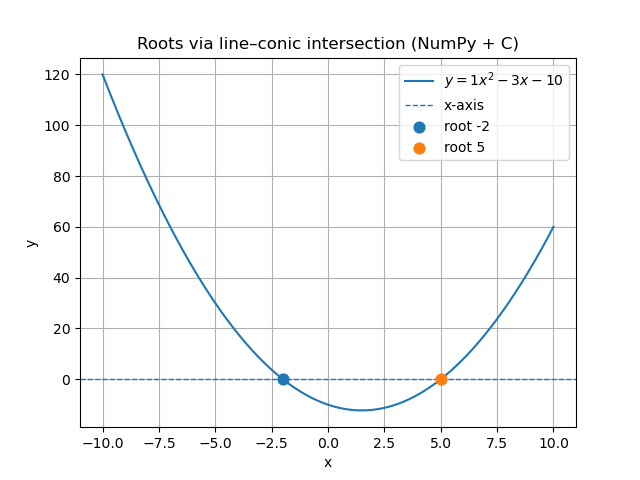
\includegraphics[width=0.9\linewidth]{figs/parabola.png}
    \caption{}
    \label{fig:placeholder}
\end{figure}


\end{document}
